\section{Results}

\subsection{Loss Distribution Separation (H-E1)}

At epoch 5, minority and majority samples show dramatically different loss distributions:

\begin{table}[h]
\centering
\begin{tabular}{@{}llll@{}}
\toprule
Statistic & Minority & Majority & Ratio \\
\midrule
Mean loss & 0.158 & 0.019 & \textbf{8.3$\times$} \\
Median loss & 0.057 & 0.001 & 57$\times$ \\
\bottomrule
\end{tabular}
\caption{Loss statistics at epoch 5 by group membership.}
\label{tab:loss_stats}
\end{table}

The Mann-Whitney U test confirms statistical significance: $U = 705,391$, $\mathbf{p = 7.36 \times 10^{-15}}$.

\begin{figure}[h]
\centering
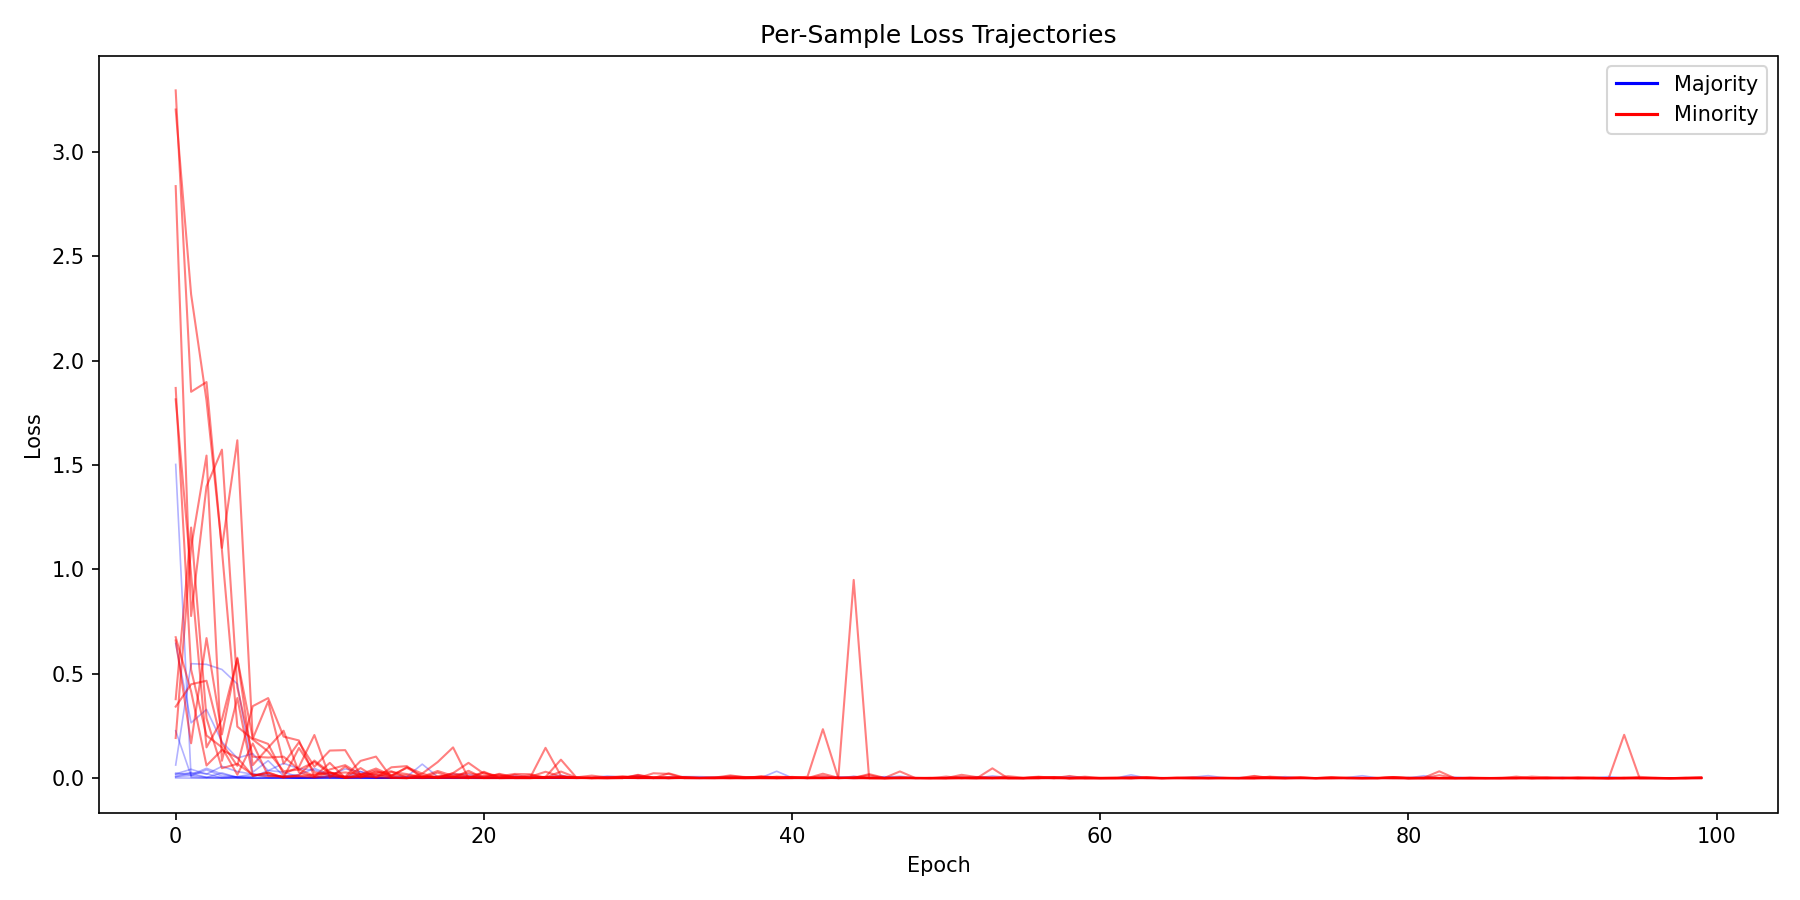
\includegraphics[width=0.8\textwidth]{figures/loss_trajectories.png}
\caption{Per-sample loss trajectories colored by group membership. Minority samples (orange) cluster in the high-loss region.}
\label{fig:loss_trajectories}
\end{figure}

\subsection{Detection Performance}

Using the 95th percentile loss threshold at epoch 5:

\begin{table}[h]
\centering
\begin{tabular}{@{}llll@{}}
\toprule
Metric & Value & Random Baseline & Lift \\
\midrule
Precision & 0.329 & 0.050 & \textbf{6.6$\times$} \\
Recall & 0.329 & 0.050 & 6.6$\times$ \\
\bottomrule
\end{tabular}
\caption{Detection performance at 95th percentile threshold.}
\label{tab:detection}
\end{table}

The 6.6$\times$ lift over random demonstrates substantial detection signal despite base-rate-limited absolute precision.

\begin{figure}[h]
\centering
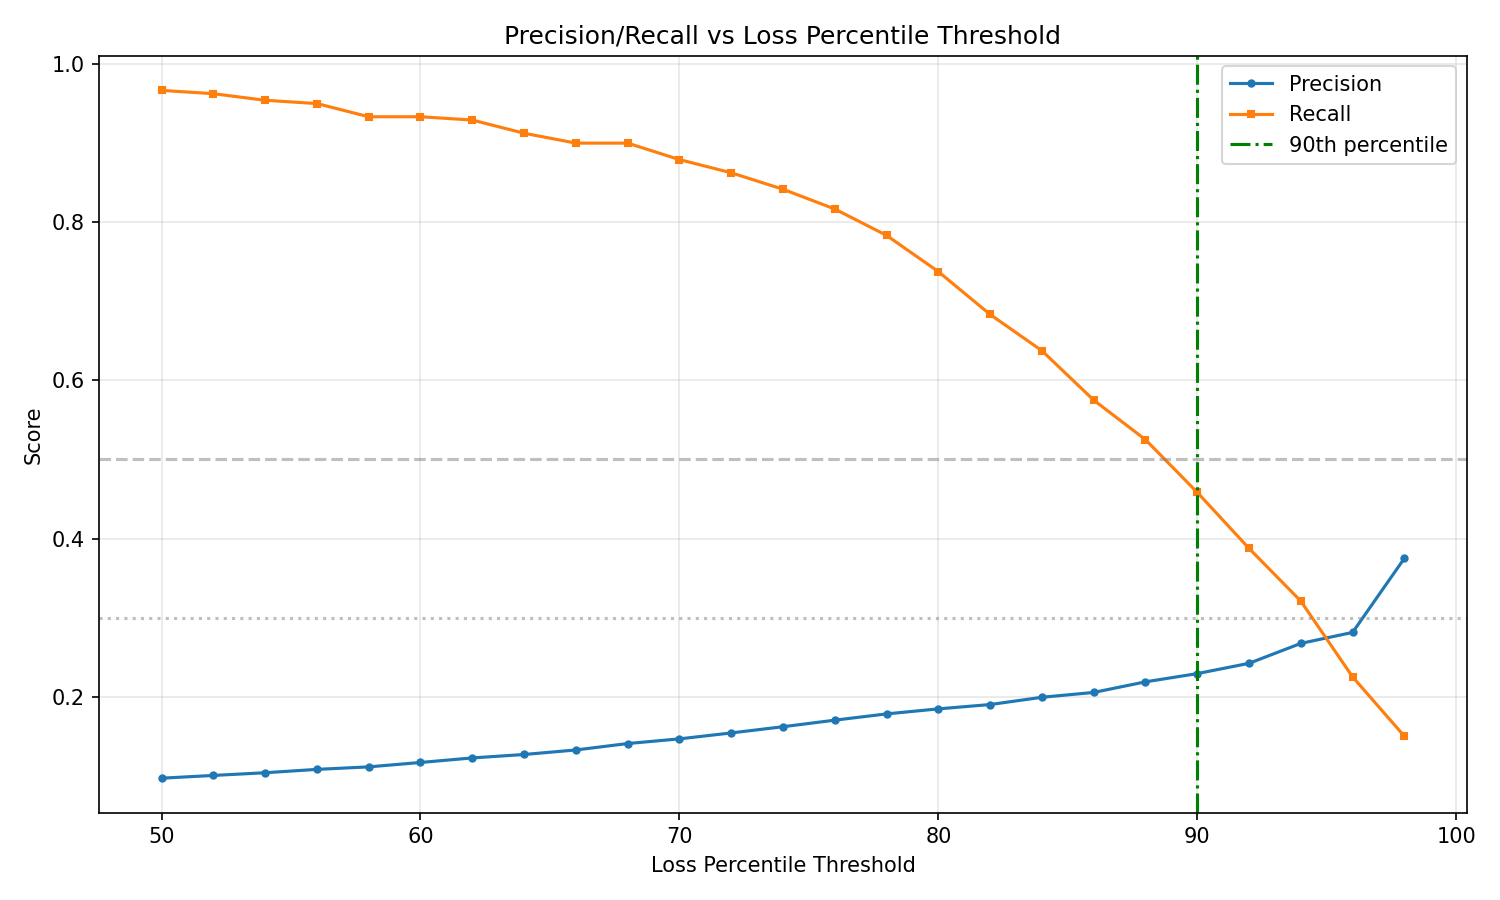
\includegraphics[width=0.8\textwidth]{figures/pr_curve.png}
\caption{Precision-recall curve for minority detection vs loss percentile threshold.}
\label{fig:pr_curve}
\end{figure}

\subsection{Simplicity Bias Mechanism (H-M1)}

Linear probe analysis confirms simplicity bias:

\begin{table}[h]
\centering
\begin{tabular}{@{}llll@{}}
\toprule
Epoch & Spurious Acc & Core Acc & Gap \\
\midrule
5 & \textbf{91.20\%} & 80.50\% & +10.70\% \\
20 & 91.59\% & 82.26\% & +9.33\% \\
50 & 91.34\% & 82.62\% & +8.72\% \\
\bottomrule
\end{tabular}
\caption{Linear probe accuracy for spurious vs core features.}
\label{tab:probe_accuracy}
\end{table}

\begin{figure}[h]
\centering
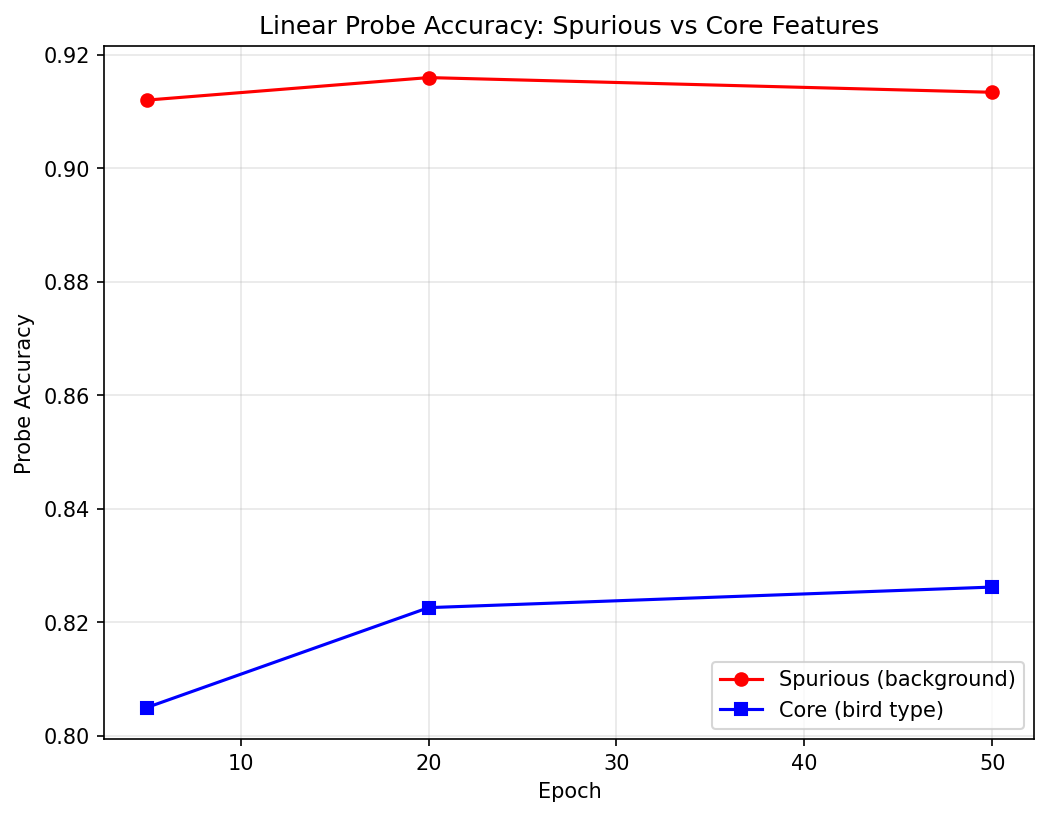
\includegraphics[width=0.8\textwidth]{figures/probe_accuracy.png}
\caption{Linear probe accuracy for spurious vs core features across epochs.}
\label{fig:probe_accuracy}
\end{figure}

\subsection{Timing Analysis (H-M2)}

Both feature types peaked at epoch 81. The timing gap hypothesis is \textbf{not supported} with pretrained features, but the magnitude gap (9--11\% throughout) confirms simplicity bias manifests differently with pretraining.

\begin{figure}[h]
\centering
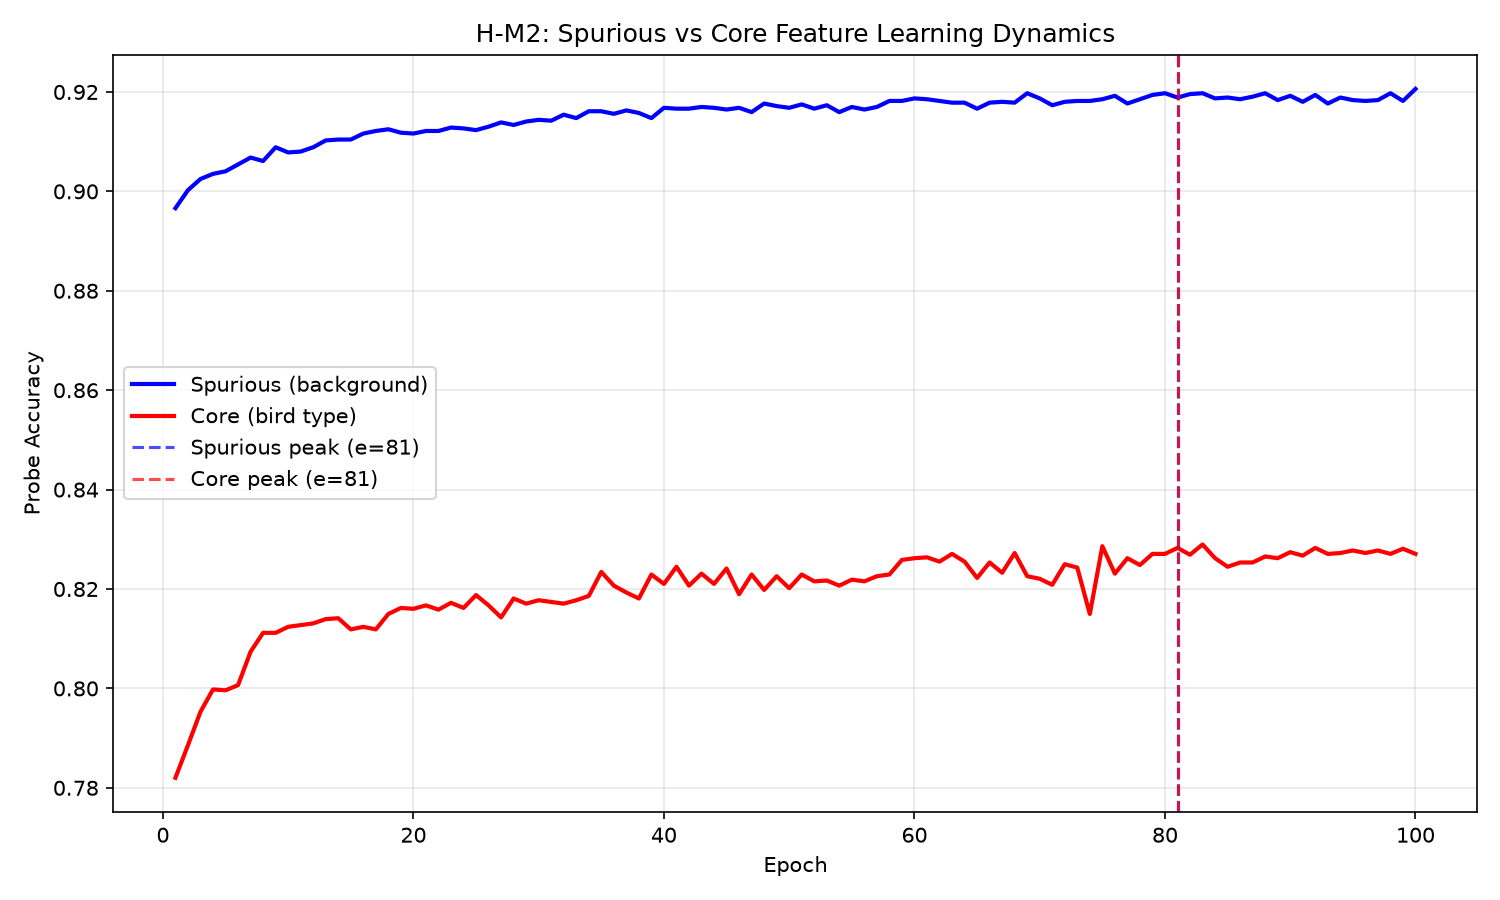
\includegraphics[width=0.8\textwidth]{figures/learning_curves.png}
\caption{100-epoch probe learning curves showing parallel trajectories with persistent magnitude gap.}
\label{fig:learning_curves}
\end{figure}
